\documentclass{article}
\usepackage[utf8]{inputenc}
\usepackage{geometry}[margins = 1in]
\usepackage{graphicx}
\usepackage{hyperref}
\usepackage{amsmath}
\usepackage{listings}
\usepackage[makeroom]{cancel}
\usepackage{color}
\usepackage{amssymb}
\usepackage{float}
\floatplacement{figure}{H}
\setkeys{Gin}{width=0.75\linewidth}

\hypersetup{
    colorlinks=true, %set true if you want colored links
    linktoc=all,     %set to all if you want both sections and subsections linked
    linkcolor=blue,  %choose some color if you want links to stand out
}


\newcommand{\unit}[1]{{\,\rm #1}}
\newcommand{\be}{\begin{equation}}
\newcommand{\ee}{\end{equation}}
\newcommand{\Mpc}{\unit{Mpc}}
\newcommand{\s}{\unit{s}}
\newcommand{\km}{\unit{km}}
\newcommand{\yr}{\unit{yr}}



\title{Extragalactic Astrophysics and Comsology}
\author{Jacob Pilawa}
\date{Spring 2021}

\begin{document}

\maketitle
\tableofcontents
\newpage

\section{The Smooth Universe}
\subsection{The Cosmological Principle; The Hubble Parameter; Scale Factor}

\subsubsection{The Cosmological Principle}

We begin with \textbf{The cosmological Principle}. It sounds simple, but incredibly well supported. It says that \textbf{the Universe (spatially) is homogeneous and isotropic on very large spatial scales}. Observationally, this is around $100 \Mpc$ scales. Homogeneous means constant density (non-realistically, this is mass density; relativistic ally, this is energy density). Isotropic means the same in all directions. 

\textit{Note}: Isotropy about $2$ points (or more) implies homogeneity. Isotropy about $1$ point is not enough. Here is a quick illustration of that: 

\begin{figure}
    \centering
    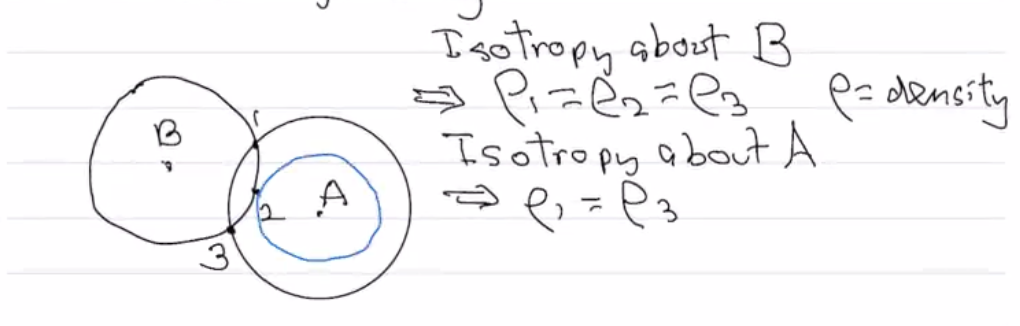
\includegraphics{isotropy.png}
    \caption{Istropy aobut 2 points.}
    \label{fig:isotropy}
\end{figure}

We can consider another example. A homogeneous universe can anisotropic. Consider a homogeneous Universe that is expanding in different directions in a non-uniform way. This leads to different $H_0(x,y,z)$. 

The reason we spend some time on the Cosmological Principle is the \textbf{Friedmann-Robertson-Walker metric}, which we will come to later on.

\subsubsection{Hubble Parameter}

Let's now talk about the \textbf{Hubble parameter}, which is not a constant! It, in fact, changes in time. An empirical linear relationship between the recession speed $v$ and distance $r$ can be seen, called the \textbf{Hubble's Law}:

\begin{equation}
v = H r
\end{equation}

Note that $H_0$ has units of $1/$time. One convention to note is that:

\begin{equation}
H = 100 \underbrace{h}_\text{to hide our ignorance} \frac{\km}{\s \Mpc}
\end{equation}

One useful number to know is $H \approx \frac{h}{10^{10} \yr}$.

Sometimes, when we write $H_0$, we mean the ``present-day'' value ($z = 0$). This is how we will use it now.

\subsubsection{Scale Factor}

We need a language to describe the expansion of the Universe. We will use $a(t)$, which describes the expansion (or contraction) of the Universe. It also relates two different coordinate systems: physical coordinates $\vec{r}$ to comoving coordinates $\vec{x}$. The relation:

\begin{equation}
    \vec{r} = a(t) \vec{x}
\end{equation}

We typically use comoving coordinates in calculations in Cosmology. We can think of $\vec{x}$ as the notches on a stretching ruler. Now consider:

\begin{equation}
    \frac{d}{dt}\vec{r} = \vec{v} = \dot{a} \vec{x} a \vec{\dot{x}}
\end{equation}

\begin{equation}
    \frac{d}{dt}\vec{r} = \vec{v} = \dot{a} \vec{x} a \vec{\dot{x}} = \underbrace{\frac{\dot{a}}{a} \vec{r}}_\text{Hubble} + \underbrace{a \vec{\dot{x}}}_\text{motion relative to expansion (``peculiar velocity'')}
\end{equation}

\begin{equation}
    \boxed{H(t) = \frac{\dot{a}(t)}{a(t)}}
\end{equation}

The name of the game for measuring $H$ is to go far enough that the first term dominates. Otherwise, locally, the second term dominates since peculiar velocities are of order $100$s of $\km/\s$. 

One other convention we need to establish:

\begin{equation}
    a(t_0) = 1 \rightarrow \text{comoving} = \text{today}
\end{equation}

\subsection{The Friedmann Equation; The Equation of State; Radiation, Matter, and Dark Energy}

\subsubsection{The Friedmann Equation}

Below, we will use and derive these, but I am putting the equations at the top for convenience. 

\begin{equation}
    \boxed{\left(\frac{\dot{a}}{a}\right)^2 = \frac{8\pi}{3} G \rho - \frac{k}{c^2}}
\end{equation}

\begin{equation}
    \boxed{\dot{\rho} = -3 \frac{\dot{a}}{a} \left(P + \rho\right)}
\end{equation}

\begin{equation}
    \boxed{\frac{\ddot{a}}{a} = - \frac{4\pi G}{3}\left(\rho +  3P\right)}
\end{equation}

Let's motivate the origin with quasi-Newtonian physics. We can derive it from General Relativity, but that's overkill.

If we assume isotropy, we only need to worry aobu the radial coordinate $r$, not $\theta$ or $\phi$. Homogeneity tells us that $\rho = \text{constant}$ spatially, but \textit{can} depend on time. We will model the Universe as an expanding, homogeneous medium that is adiabatically ($\Delta s =0$) expanding. If it were not adiabatically expanding, we would have heat flow and thus no isotropy. 

With these conditions, let's examine the motion of a thin, expanding, spherical shell of radius $a$. This depends \textbf{only} on the enclosed mass within $a$\footnote{see Birkhoff's Theorem for General Relativity proof}:


\begin{equation}
    M(<a) = \frac{4}{3}\pi a^3 \rho
\end{equation}

Let's consider the energy:


\begin{equation}
    E = \frac12 \dot{a}^2 - \frac{GM}{a}
\end{equation}


\begin{equation}
E = \frac12 \dot{a}^2 - \frac43 \pi G \rho a^2
\end{equation}

Let's re-write $E$ a bit: $k c^2 \equiv -2E$. Note that $k \propto 1/\text{length}^2$. There are three possibilities for $kc^2$:

\begin{itemize}
    \item $>0$, $E<0$, bound
    \item $=0$, $E=0$, critical
    \item $<0$, $E>0$, unbound
\end{itemize}

Let's now evoke the First Law of Thermodynamics ($\Delta S = 0$):

\begin{equation}
   \underbrace{\mathrm{d}U}_\text{internal energy} = -P \mathrm{d}V 
\end{equation}

We now equation the internal energy to the rest-mass energy:

\begin{equation}
    \mathrm{d}\left(\rho c^2 a^3\right) = -P \mathrm{d}\left(a^3\right)
\end{equation}

We will now set $c = 1$ and take a time derivative:

\begin{equation}
    \dot{\rho} a^3 + 3 \rho a^2 \dot{a} = -3P a^2 \dot{a}
\end{equation}

\begin{equation}
    \dot{\rho} -3\frac{\dot{a}}{a}\left(P + \rho\right)
\end{equation}

Using this result and the energy equation from above

\begin{equation}
    \left(\frac{\dot{a}}{a}\right)^2 = \frac{8\pi}{3}G \rho - \frac{k (c)^2}{a^2}
\end{equation}

to get a new equation. If you stare at it hard enough and have divine intervention, take a derivative of the second equation and multiply by $a^2$. Doing so, you get:

\begin{equation}
    2 \dot{a} \ddot{a} = \frac{8\pi}{3}G\frac{d}{dt}(\rho a^2) = \frac{8\pi}{3}Ga^2\left(\dot{\rho} + 2\frac{\dot{a}{a}}\rho\right)
\end{equation}

Simplifying with the other above equation, we get:

\begin{equation}
    2\dot{a}\ddot{a} = -\frac{8\pi}{3}Ga^2 \left(\frac{\dot{a}}{a}\rho + 3\frac{\dot{a}}{a}P\right)
\end{equation}

Simplifying:

\begin{equation}
    \frac{\ddot{a}}{\dot{a}} = -\frac{4\pi}{3}G \left(\rho + 3P\right)
\end{equation}

Note that this is not independent from the other equations; rather it is massaged. Let's compare this to $1$-D Newtonian forces:

\begin{equation}
    \ddot{x} = -\frac{GM}{x^2} = -\frac{4}{3}\pi G \rho x
\end{equation}

\begin{equation}
    \frac{\ddot{x}}{x} = -\frac{4}{3}\pi G \rho 
\end{equation}

Had we done strictly Newtonian physics, we would have never gotten the $+3P$ term. The way to interpret this: we can think of $\rho$ to have an extended meaning: $\rho_{eff} = \rho + 3P$. 

The Grand Summary so far: two equations of motion for $a(t)$: 

\begin{equation}
    \frac{\ddot{a}}{\dot{a}} = -\frac{4\pi}{3}G \left(\rho + 3P\right)
\end{equation}

\begin{equation}
    \dot{\rho}= -3\frac{\dot{a}}{a}\left(P + \rho\right)
\end{equation}

Note this second equation tells us the acceleration! Very importantly, we have a minus sign. If $\rho$ and $P$ are positive, the Universe is \textbf{decelerating}! Conversely, if you have a \textit{bizarre} $P$ and could reverse the parenthetical term, we can have accelerated expansion! 


Right now, we have three unknowns ($P, \rho, a$). How do we get that last piece -- the equation of state ($P \iff \rho$ dependence)?

\subsubsection{Equation of State}

We choose to write:

\begin{equation}
    P = w\rho (c^2)
\end{equation}

We are in units where $c = 1$, but I threw it in for reference. Note -- this means that pressure is the same thing as energy density! Think of the units. 

With that definition of $P$, we can re-write the second boxed equation from above:

\begin{equation}
    \dot{\rho} -3\frac{\dot{a}}{a}\left(1+w\right)\rho
\end{equation}

\begin{equation}
    \frac{\dot{\rho}}{\rho} = -3 (1+w) \frac{\dot{a}}{a} \rightarrow \rho \propto a ^{-3(1+w)}
\end{equation}

\begin{equation}
    \boxed{\rho \propto a^{-3\left(1+w\right)}}
\end{equation}

\textbf{assuming that} $\dot{w} =0$ \textbf{which might not be true}!

\subsubsection{Matter, Radiation, and Dark Energy}

Let's look at a few special cases of the equation of state:

\begin{itemize}
    \item Matter: Non-relativistic, pressure-less particles like cold dark matter. In this case, $w = 0, P = 0 \rightarrow \boxed{\rho \propto a^{-3}}$. This makes sense because it is units of $1/\text{volume}$.
    \item Radiation: Relativistic particles, photons and neutrinos. In this case, $w = 1/3, P = \frac13 \rho \rightarrow \boxed{\rho \propto a^{-4}}$. This makes sense because it is units of $\left(1/\text{volume}\right)\left(1/\text{length}\right) $ where the extra factor is from redshifting energy.
    \item The Cosmological Constant: In this case, $w = -1, P=-\rho \rightarrow \rho = \text{constant}$.
    \item Dark Energy: More general term, where $w < -\frac13$ to make $\ddot{a} >0$.
\end{itemize}

\begin{figure}
    \centering
    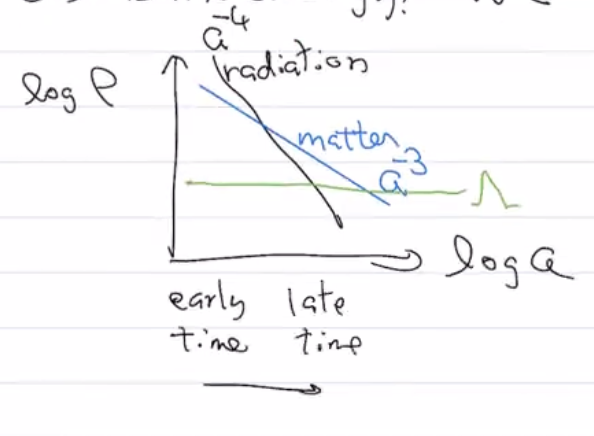
\includegraphics{density.png}
    \caption{Sketch of density over cosmic time. }
    \label{fig:density}
\end{figure}


\end{document}
